\documentclass[border=5mm]{standalone}
\usepackage{tikz}
\usetikzlibrary{calc, intersections}

\begin{document}
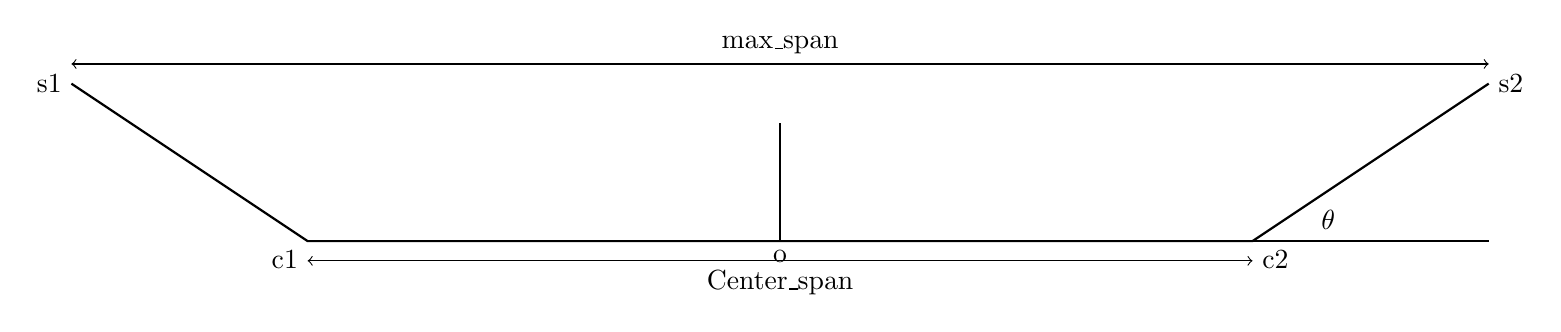
\begin{tikzpicture}

  \coordinate [label=below:o] (o) at (0,0); % name the origin
  \coordinate [label=left:s1] (s1) at (-9,2); % left tip
  \coordinate [label=right:s2] (s2) at (9,2);
  \coordinate [label=below left:c1] (c1) at (-6,0); % left center span
  \coordinate [label=below right:c2] (c2) at (6,0);  % right center

  \draw[thick] (s1) -- (c1) -- (c2) -- (s2);
  \draw[thick] (o) -- (0,1.5);
  \draw[thick] (c2) -- ($ (c2) + (3,0) $);
  \node at ($ (c2)+(16:1)$) {$\theta$};
  \draw[<->] ($ (s1)+(0,0.25) $) -- node[above] {max\_span} ($ (s2)+(0,0.25) $);
  \draw[<->] ($ (c1)+(0,-0.25) $) -- node[below] {Center\_span} ($ (c2) + (0,-0.25) $);
\end{tikzpicture}
\end{document}

